%!TEX root =  ./JanasJanssenCuffaro-August2019.tex

%SUBSUBSECTION 3.2.4
\subsubsection{Spin-$s$ ($s \ge 2$)}  \label{2.2.4}

To simulate the correlations found by measurements on a singlet state of two spin-2 particles, we use  tickets with five outcomes $\pm 2,\pm 1,0$. This results in 63 relevant ticket types, corresponding to a $62$-dimensional simplex of raffles. The conditions for uniform marginals and cell symmetry yield six linear constraints, yielding a 50-dimensional polytope of admissible raffles in 63-dimensional space. Unfortunately, the number of vertices determined by these conditions is daunting: If we consider only the six conditions for uniform marginals, computer calculation produce 553,664 vertices. This is already orders of magnitude larger than the vertex sets for the earlier polytopes. The full case, obtained by including the six conditions for cell symmetry, is presumably even larger but we have not been able to run the vertex enumeration algorithm to completion on a personal computer. Hence we do not know how many vertices the spin-$2$ admissible polytope has, much less the full list of such. This computational obstacle only grows worse as the spin increases, as is evident from the numbers in Figure \ref{numberoftickets}. The enumeration of basic admissible raffles thus becomes intractable for spin $s\geq 2$. As a consequence, the flowchart in Figure \ref{flowchart} comes to a halt and we cannot hope to compute the anti-correlation polyhedron in the way it depicts.

\begin{figure}[ht]
 \centering
   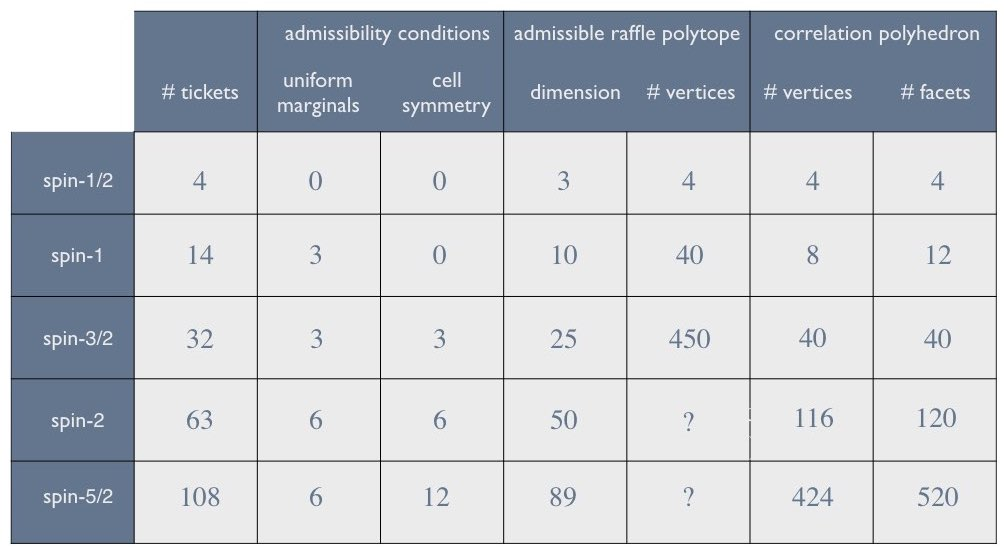
\includegraphics[width=4.5in]{numberoftickets.jpeg} 
   \caption{Number of ticket types, admissibility conditions, and facet/vertex counts for polytopes and polyhedra up to spin-$\frac52$.}
      \label{numberoftickets}
\end{figure}

Fortunately, there is an alternative approach which---while it does not yield the full polytope---does allow us to characterize the polyhedron of anti-correlation coefficients. As a first step we observe that, for every spin considered so far, the  polyhedron of anti-correlation coefficients always at least contained the spin-$\frac12$ classical tetrahedron. This is not a  coincidence. For instance, consider the point $\vec{\chi}=(1,1,1)$ where all outcomes are perfectly anti-correlated. There is actually a simple construction of an admissible spin-$s$ raffle with such behavior. To do so, it is convenient to introduce the following notation for the remainder of this section: Let $[m_a,m_b,m_c]$ denote the ticket type for which the outcomes $m_a,m_b,m_c$ for settings $\hat{a},\hat{b},\hat{c}$ appear on one side. As usual, we regard $[-m_a,-m_b,-m_c]$ as equivalent to $[m_a,m_b,m_c]$.

With this notation in mind, consider the spin-$s$ raffle (with $2s+1$ outcomes $m=-s$ to $s$) containing one of each of the tickets $$[s,s,s], [s-1,s-1,s-1], \cdots, [-s+1,-s+1,-s+1], [-s,-s,-s].$$ Since each of these ticket types appears once, the raffle has uniform marginals. If we swap any two settings on every ticket, all tickets are unchanged and therefore the raffle is cell-symmetric. Hence this raffle is admissible. As every outcome on one side of each ticket is strictly anti-correlated with every outcome on the other side, we obtain $\chi_{ab}=\chi_{ac}=\chi_{bc}=1$.

Thus for any spin there is an admissible raffle for which $\vec{\chi}=(1,1,1)$. The other three points then follow by symmetry: We take each ticket type and swap all outcomes for a given setting (e.g., take the outcomes for setting $\hat{a}$ to range from $-s$ to $+s$). This generates three more admissible raffles, characterized by $\vec{\chi}=(-1,-1,1)$, $(-1,1,-1)$, $(1,-1,-1),$ respectively. Hence all four vertices of the classical tetrahedron can be produced by admissible raffles regardless of the number of outcomes. By convexity, it follows that the anti-correlation polyhedron always includes the entire classical tetrahedron.

In general, however, the classical tetrahedron is not the full polyhedron. To establish this, we again recall that the points $\vec{\chi}=(-1,-1,1)$, $(-1,1,-1)$, $(1,-1,-1)$ generate a facet of the classical tetrahedron. This would correspond to the Bell inequality $\chi_{ab}+\chi_{ac}+\chi_{bc}\geq -1$. But, as we have shown for spin $1$ through $\frac32$, there exist admissible raffles that violate this inequality. 
\begin{table}[ht]
\centering
\begin{tabular}{|c|c|}
\hline
Ticket  & Ticket \\
fractions & types \\[.1cm]
\hline
$f^1$ & $[0,0,0]$ \\[.2cm]
$f^2$ & $[0,1,-1]$ $[1,0,-1]$ $[1,-1,0]$ \\[.2cm]
$f^3$ & $[0,1,-1]$ $[1,0,-1]$ $[1,-1,0]$ \\[.2cm]
$f^4$ & $[0,1,-1]$ $[1,0,-1]$ $[1,-1,0]$ \\[.2cm]
\hline
\end{tabular}
\caption{Ticket types and ticket fractions for the four ticket groups used to construct admissible raffles which maximally violate the Bell inequality. Each ticket type in a given group occurs with the same frequency in the full raffle.}
\label{Spin2TicketGroups}
\end{table} 

Suppose we now focus on finding admissible raffles which maximally violates this inequality. One approach exploits the observation made in Section \ref{1.6}: To violate the Bell inequality as strongly as possible, we should use ticket types which render $(X_a^A+X_b^A+X_c^A)^2$ as small as possible. For integer spin, this suggests restricting attention to those ticket types whose outcomes sum to zero on the left side (and so also the right side). In the case of spin 2, only 10 out of the 63 tickets to fulfill this criterion. Enforcing cell symmetry on this limited subset of tickets results in the four groups of ticket types shown in Table \ref{Spin2TicketGroups}. For a raffle to be cell-symmetric requires that the fraction of tickets of a given type be the same for all members of a group. We denote these common ticket fractions as $f^1,f^2,f^3,f^4$ for the four respective ticket groups. Enforcing uniform marginals then yields the conditions (cf.\ Eqs.\ (\ref{adm spin1 diag})-(\ref{spin 1 constraints})) 
% \begin{align}
% \text{Pr}(m_1=2|\hat{a})&=&\text{Pr}(m_1=2|\hat{b})=\text{Pr}(m_1=2|\hat{c})= f^3+\frac12 f^4=\frac15, \\
% \text{Pr}(m_1=1|\hat{a})&=&\text{Pr}(m_1=1|\hat{b})=\text{Pr}(m_1=1|\hat{c})= f^2+\frac12 f^1=\frac15,\\
% \text{Pr}(m_1=0|\hat{a})&=&\text{Pr}(m_1=0|\hat{b})=\text{Pr}(m_1=2|\hat{c})= f^1+f^2+f^3=\frac15,
% \end{align}
$$f^1+f^2+f^3=f^2+f^4=f^3+\sfrac12 f^4=\sfrac15.$$ These four equations in three unknowns have a one-dimensional solution set. It can then be shown that the subset of non-negative solutions is generated by convex combinations of the following:

\begin{itemize}
    \item $(f^1,f^2,f^3,f^4)=(\sfrac{1}{10},0,\sfrac{1}{10},\sfrac{2}{10})$, corresponding to a raffle with tickets
    \begin{equation*}
    \begin{array}{*{5}c}
        {[0,\;\, 0,\;\, 0]}  & {[2,0-2]} & {[1,1,-2]} & {[1,-2,1]} & {[2,-1,-1]} \\
        {[0,2,-2]} & {[2,-2,0]} & {[1,1,-2]} & {[1,-2,1]} & {[2,-1,-1]}
    \end{array}
    \end{equation*}
    \item $(f^1,f^2,f^3,f^4)=(0,\sfrac{1}{15},\sfrac{2}{15},\sfrac{1}{15})$, corresponding to a raffle with tickets
    \begin{equation*}
    \begin{array}{*{5}c}
        {[0,1,-1]} & {[0,2,-2]} & {[2,0,-2]} & {[1,1,-2]} & {[1,\;\, -2,\;\, 1]}  \\
        {[1,0,-1]} & {[0,2,-2]} & {[2,-2,0]} & {[1,1,-2]} & {[2,-1,-1]} \\ 
        {[1,-1,0]} & {[2,0-2]} & {[2,-2,0]} & {[1,-2,1]} & {[2,-1,-1]}
    \end{array}
    \end{equation*}
\end{itemize}

% Do not remove the curly brackets. Otherwise, Latex interprets [x] to be a dimension (e.g. [cm]) and will not compile properly.

% \begin{table}[ht]
% \centering
% \begin{tabular}{|c|*{5}c|}
%     \hline
%     $(f^1,f^2,f^3,f^4)$ & & & Admissible raffle & & \\
%     \hline \\
%     $(\sfrac{1}{10},0,\sfrac{1}{10},\sfrac{2}{10})$
%         & {[0,0,0]}  & {[0,2,-2]} & {[2,0,-2]} & {[2,-2,0]} & {[1,1,-2]} \\
%         & {[1,1,-2]} & {[1,-2,1]} & {[1,-2,1]} & {[2,-1,-1]} & {[2,-1,-1]} \\ \\
%     \hline \\
%     $(0,\sfrac{1}{15},\sfrac{2}{15},\sfrac{1}{15})$
%         & {[0,1,-1]} & {[1,0,-1]} & {[1,-1,0]} & {[0,2,-2]} & {[0,2,-2]}  \\
%         & {[2,0,-2]} & {[2,0,-2]} & {[2,-2,0]} & {[2,-2,-0]} & {[1,1,-2]} \\ 
%         & {[1,1,-2]} & {[1,-2,1]} & {[1,-2,1]} & {[2,-1,-1]} & {[2,-1,-1]}\\
%     \hline
% \end{tabular}
% \caption{}
% \label{}
% \end{table} 

One may confirm that, in keeping with the ticket outcomes all summing to zero, both raffles map to the point $\vec{\chi}=(-\sfrac12,-\sfrac12,-\sfrac12)$. We have thus gone from a 50-dimensional polytope of admissible raffles to a 1-dimensional subspace of such raffles, all of which maximally violate the Bell inequality.\footnote{These raffles validate that, for spin up to $2$, we can always find an admissible raffle while using only tickets which minimize the magnitude of $X_a^A+X_b^A+X_c^A$. This is actually true in general: For any spin, there is a procedure to construct an admissible raffle using only tickets which minimize $(X_a^A+X_b^A+X_c^A)^2$. This construction, however, is somewhat involved and moreover beyond the scope of the present work, so we do not pursue this line further.}

%For half-integer spin, the smallest magnitude which $X_a^A+X_b^A+X_c^A$ can achieve is now 1/2 rather than 0. This still restricts the set of allowed tickets substantially. For instance, in the case of spin $5/2$ there are six outcomes and therefore $6^3/2=108$ relevant ticket types. However, there are only 27 tickets for which the sum of outcomes has magnitude $1/2$. Imposing the admissibility conditions reduces this 26-dimensional subspace of raffles further. What results is an 11-dimensional polytope of admissible raffles, generated as the convex hull of 288 vertices. Mapping these 288 vertices to their anti-correlation coefficients yields the point set shown in [Figure], all of which lie on the plane $$\chi_{ab}+\chi_{ac}+\chi_{bc} = -\frac{3}{2}+\frac{3}{35}$$ which [as per the deFinetti section] represents the maximum possible violation of the Bell inequality for spin $5/2$. From this point set we obtain 15 vertices, and the convex hull of these 15 vertices is a facet of the anti-correlation polyhedron.

We have thus obtained another vertex of our spin-2 polyhedron, one which lies beyond the facet of the classical tetrahedron opposite the point $\vec{\chi}=(1,1,1)$. By exploiting the tetrahedral symmetry of the anti-correlation coefficients, we obtain three other such vertices that lie beyond the other three facets. Invoking convexity again, we obtain another polyhedron of admissible anti-correlation coefficients which is larger than the classical tetrahedron (though still necessarily bounded by the elliptope) and therefore more closely `approximates' the full anti-correlation polyhedron.

At this point, there is nothing in principle to stop us from pursuing the following strategy, which is essentially the convex hull algorithm of \citet{Lassez and Lassez 1992}. We start with some `approximate' polyhedron, such as the classical tetrahedron, which the true anti-correlation polyhedron contains. We pick one of the facets of the approximate polyhedron, and determine whether any admissible raffles exist which violate the corresponding linear inequality on anti-correlation coefficients. If no such raffle exists, we conclude that the facet under consideration is indeed a facet of the anti-correlation polyhedron and we move on to another facet. If such a raffle does exist, however, we determine one which maximally violates the corresponding inequality. The resulting set of anti-correlation coefficients will be an extreme point of the anti-correlation polyhedron. We then invoke convexity and enlarge our approximate polyhedron to include this new extreme point, thereby obtaining a better approximation of the anti-correlation polyhedron. This algorithm terminates when every facet of the approximate polyhedron is verified to be a facet of the anti-correlation polyhedron, at which point we conclude that the entire polyhedron has been generated.

The hardest step in this method is to determine whether any admissible raffles map to points beyond a given facet. One approach would be to imitate the strategy outlined for the case of $\chi_{ab}+\chi_{ac}+\chi_{bc}$: For each linear inequality, we determine a corresponding linear relation $v_a X_a^A+v_b X_b^A+v_c X_c^A$ and look for admissible raffles using only tickets for which this quantity has small magnitude, thereby ensuring that the facet inequality is violated as strongly as possible. Take, for example, the spin-$2$ case. We have shown that its anti-correlation polyhedron contains the points  $(-1,1,-1)$, $(1,-1,-1)$, and $(-\sfrac12,-\sfrac12,-\sfrac12)$. The plane through these three points is given by $\chi_{ab}+\chi_{ac}+2\chi_{bc}=-2$. We want to determine whether this gives a facet. Observing that 
\begin{equation}
\big\langle \left(X_a^A+2X_b^A+2X_c^A\right)^2\big\rangle  = 18+8 \, (\chi_{ab}+\chi_{ac}+2\chi_{bc}),
\end{equation}
we are led to consider tickets for which $(X_a^A+2X_b^A+2X_c^A)^2$ is small in order to minimize $\chi_{ab}+\chi_{ac}+2\chi_{bc}$. Proceeding in this way, we ultimately obtain all admissible raffles which are characterized by the seven-sided facet at the bottom of Figure \ref{FacetsSpin2Spin52}.

There are, however, several problems with this method. The first is that it is necessarily somewhat tedious: The linear relation to be minimized must be computed for each facet under consideration, and therefore will lead to different sets of tickets in each case. Second, it is not obvious how many tickets one will need to successfully produce admissible raffles. In the case of spin 2, there are 7 tickets for which this expression is zero and 9 for which it has magnitude 1; it turns out that we need to use tickets of both magnitudes to get an admissible raffle. This is still far smaller than the 63 ticket types total, but it is not nearly as attractive as the 10 tickets with outcomes summing to zero in the $\chi_{ab}+\chi_{ac}+\chi_{bc}$ case. Finally, and most importantly, our iterative strategy only needs one admissible raffle that maximally violates the relevant facet inequality. It is therefore altogether excessive to characterize the entire set of such admissible raffles for a given facet.

\begin{figure}[ht]
 \centering
   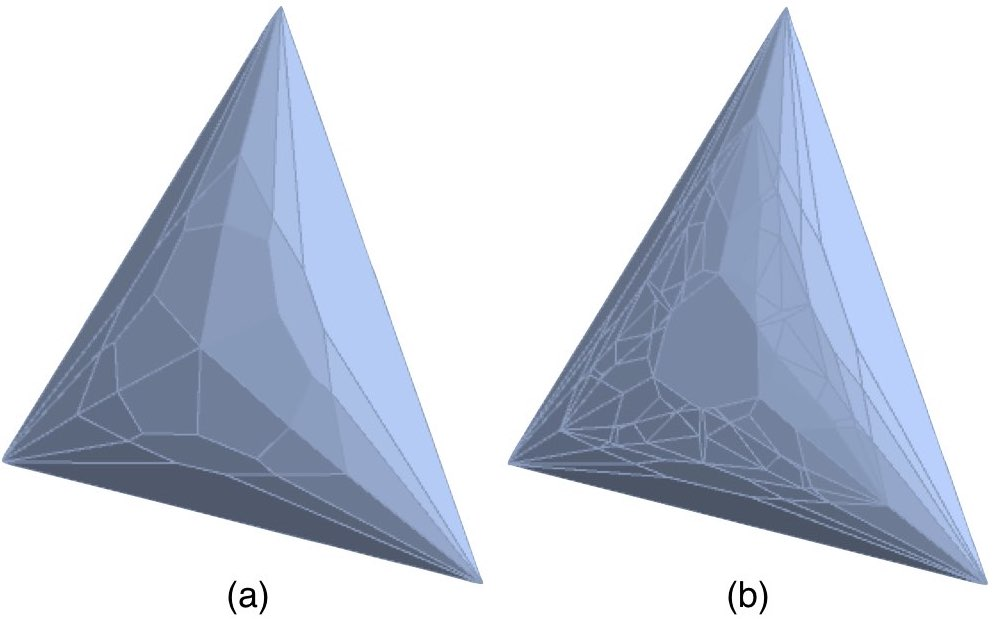
\includegraphics[width=4.5in]{FacetsSpin2Spin52.jpeg} 
   \caption{Facet of polyhedron for (a) spin-$2$ and (b) spin-$\frac52$ (cf.\ Figure \ref{SpinThreeHalfFace}).}
   \label{FacetsSpin2Spin52}
\end{figure}

Rather than pursue this approach further, we will instead exploit the well-known connection between polytopes and \emph{linear programming} \citep{Dantzig and Thapa 1997, Dantzig and Thapa 2003}. We consider a spin-$s$ raffle and let $\Delta^{n-1}$ be the appropriate $(n-1)$-dimensional simplex of raffles, where $n$ is the number of relevant ticket types. Since all the admissibility conditions are all linear in the ticket fractions, we may conveniently express them in the form $B\vec{f}_{\mathrm{adm}}=\vec{b}$; the matrix $B$ and the vector $\vec{b}$ will have as many rows as there are (linearly independent) constraints. Finally, the linear function to be minimized can be expressed as $\vec{c}\cdot \vec{\chi}|_{\vec{f}_{\mathrm{adm}}}$ for some real 3-vector $\vec{c}$. This \emph{objective function} is in terms of the anti-correlation coefficients, but as before the mapping of ticket fractions to anti-correlation coefficients is expressed as $\vec{\chi}|_{\vec{f}_{\mathrm{adm}}}=M\vec{f}_{\mathrm{adm}}$ where $M$ is a $3\times n$ matrix. Hence the objective function may be written in terms of ticket fractions:
\begin{equation}
    \vec{c}\cdot \vec{\chi}|_{\vec{f}_{\mathrm{adm}}}=\vec{c}\cdot (M\vec{f}_{\mathrm{adm}})=(M^\top \vec{c})\cdot \vec{f}_{\mathrm{adm}}.
\end{equation}
To maximally violate a particular facet inequality, then, is equivalent to minimizing this objective function over the set of $\vec{f}_{\mathrm{adm}}\in \Delta^{n-1}$ satisfying $B\vec{f}_{\mathrm{adm}}=\vec{b}$. The problem of finding such an admissible raffle therefore takes the form of a particular \emph{linear program},  and thus our iterative strategy requires the solution of a finite number of linear programs. Such linear programs can be solved via the so-called simplex method at relatively low computational cost. In this way, we implemented our iterative strategy in Mathematica and so obtain an algorithm to compute all vertices of the anti-correlation polyhedron. The resulting local polyhedra, in the case of spin-$2$ as well as spin-$\frac52$, appear in Figure \ref{FacetsSpin2Spin52}. As in Figure \ref{SpinThreeHalfFace}, this picture shows the facets we need to ``glue onto" each of the four facets of the classical tetrahedron to get the full polyhedron.

\begin{figure}[ht]
 \centering
   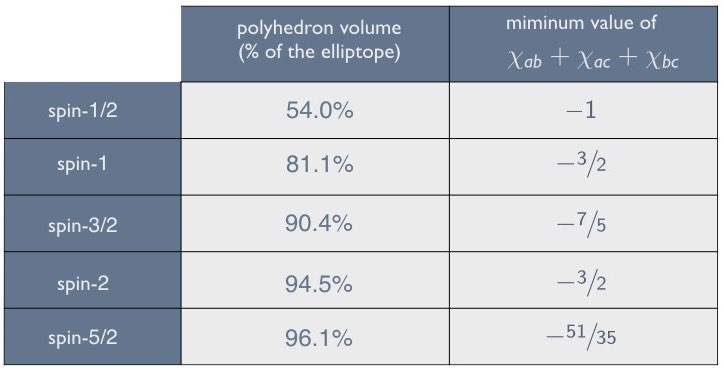
\includegraphics[width=4.5in]{polytopevolume.jpeg} 
   \caption{Polytope volumes and minimal values of the sum of anti-correlation coefficients}
   \label{polytopevolume}
\end{figure}

The anti-correlation polyhedra presented thus far (Figures \ref{tetrahedron}, \ref{polytope-spin1}, and \ref{SpinThreeHalfFace}) suggests that, as the number of outcomes increases, the anti-correlation polyxhedron converges to the full elliptope. This is not really surprising, for if we were to allow for a continuous range of outcomes rather than a discrete set then the full elliptope of correlation matrices is certainly generated. Indeed, for the case of a multivariate Gaussian distribution, the probability distribution is parametrized by the choice of a positive-definite correlation matrix.\footnote{A simpler example is provided by the \emph{3m balance} discussed in Section \ref{1.6.4} (see Figure \ref{3M-balance})).\label{3M convergence}} Thus the failure to obtain the full elliptope rests on the discrete nature of the outcomes.\footnote{One could say that the \emph{discreteness} introduced by quantum mechanics puts some restrictions on the elliptope but that those restrictions are lifted again by the \emph{contextuality} it introduces.\label{discrete and contextual}}  As numerical evidence for convergence we consider the volume of our polyhedra, which can be computed from the list of vertices. These volumes are listed in Figure \ref{polytopevolume} in terms of their fraction of the elliptope volume (which may be shown to be exactly $\pi^2/2$). These volumes are seen to increase monotonically to that of the full elliptope as spin increases, in agreement with the convergence we are seeing in the figures.\footnote{The admissibility conditions on the correlations represented by points in our correlation polyhedra form the main obstacle to a formal proof of this convergence. As we saw in Section \ref{2.2.3}, these conditions are of two kinds: the correlations should have uniform marginals and their correlation arrays should have the same symmetries as the quantum-mechanical ones they are meant to simulate. The convergence issue can meaningfully be studied without these symmetry conditions. The uniform-marginals condition, however, is critical for the construction of our correlation polyhedra. For one thing, as already mentioned in the introduction to Section \ref{2}, we need this condition to ensure that the correlation arrays in some allowed class differ only in their off-diagonal cells.\label{no-convergence-proof}}


